\chapter{Aquifer specification\label{cha:aqu-module}}

The aquifer module (AQU) is used to define the layout and properties of the ModAEM aquifer. In ModAEM, an aquifer is considered to be a single, horizontal, two-dimensional flow system. A ModAEM aquifer may be bounded or unbounded spatially, with a variety of boundary conditions specified at the perimeter of the bounded domain. All aquifers in ModAEM may have heterogeneous hydraulic conductivity, base elevation, thickness and porosity, specified in inhomogeneities. An inhomogeneity is a bounded sub-region of the aquifer where the hydraulic properties of the aquifer differ from the surrounding region. In ModAEM, inhomogeneities may be nested within other inhomogeneities, and may share common boundaries.

\section{Aquifers in ModAEM}

Like most analytic element models, ModAEM supports heterogeneous aquifers in which aquifer properties are constant within polygonal domains (aquifer properties are ``piecewise--constant''). In ModAEM, each sub-domain may have its own aquifer base and top elevation, hydraulic conductivity, and porosity.

\section{AQU Module Input }

As with all other modules that are included in the problem definition section of a ModAEM script file, input for module AQU is contained between the \textsf{aqu} directive and the \textsf{end} directive. Module AQU differs from some of the other ModAEM modules, in that it posesses optional submodules. The general layout for module AQU input is as follows:
\begin{verbatim}
\# Create an aquifer
aqu ndomains nstrings base thickness conductivity porosity
  ref <arguments> (optional) define a reference point and discharg
  bdy <arguments>
    (optional) define flow conditions at the perimeter 
  end 
  in0 <arguments>
    (optional) define inhomogeneities 
  end
end
\end{verbatim}
The remainder of this section describes the detailed usage of the
AQU module directives.

\subsection{Beginning the aquifer definition (directive \textsf{aqu})}

The \textsf{aqu} directive starts the process of defining the aquifer
layout. In addition to the regional aquifer properties, the aqu directive
allocates space for the definition of subdomains of differing aquifer
properties, and boundary conditions for bounded models.

\paragraph{Usage:}
\begin{verbatim}
  aqu ndom nstr bot thick hyd-cond poro avg-head
\end{verbatim}

\paragraph{Parameters for the \textsf{\textmd{aqu}} directive:}
\begin{description}
\item [{\texttt{ndom}} (int)] The number of inhomogeneity domains in the aquifer, including the outside unbounded domain. For a single homogeneous aquifer, use 1. $[-]$
\item [{\texttt{nstr}} (int)] The number of strings that are used to bound the inhomogeneity domains. For a single inhomogeneous aquifer, use 0. $[-]$
\item [{\texttt{bot}} (real)] The base elevation of the aquifer $[\mathrm{L}]$
\item [{\texttt{thick}} (real)] The thickness of the aquifer $[\mathrm{L}]$
\item [{\texttt{hyd-cond}} (real)] The hydraulic conductivity of the aquifer $[\mathrm{L/T}]$
\item [{\texttt{poro}} (real)] Porosity of the aquifer as a fraction $[-]$
\item [{\texttt{avg-head}} (real)] This is an estimate of the average head in the aquifer. It is used to pre--condition the solution when inhomogeneities in base elevation or thickness are encountered and the flow condition is unconfined. If you expect to be using inhomogeneities in base elevation or aquifer thickness, a good estimate of the initial average head will greatly speed the solution process. If you are not using inhomogeneities in base elevation or aquifer thickness, it is recommended that the value of $\mathtt{bot+thick}$ be provided. $[\mathrm{L}]$
\end{description}

\paragraph{Simple Aquifer Example }

To build a simple infinite aquifer with no inhomogeneities, with base elevation at $0\mathrm{\ ft}$, thickness of $10\mathrm{\ ft}$, hydraulic conductivity of $100\mathrm{\ ft/d}$, porosity of $0.25$ and an average head of $200\mathrm{\ ft}$,
only one domain and no strings are required. The \textsf{aqu} directives
\begin{verbatim}
  aqu 1 0 0.0 10.0 100.0 0.25 200.0
  end
\end{verbatim}
will create this aquifer.

\subsection{Defining a reference flow field (directive \textsf{ref})
\label{sub:reference-flow-field}}

ModAEM differs from some analytic element codes in that the specification of a reference point is often unnecessary. Typically, the reference flow field is only needed in conceptual models or when a site--scale model based on a uniform flow field has been measured in the field.

\paragraph{What is the reference flow field?}

In an analytic element model, it is possible to define a problem in which all of the elements (wells, etc.) possess a specified discharge (e.g. the common conceptual model of one or more wells in a uniform flow field). In these cases, a unique solution can be generated only if the user specifies a point in the aquifer at which the head is known. Specification of the reference point enables the specification of a reference flow field, a uniform flow discharge that will be present everywhere in the aquifer, even if no elements are present. The reference flow field is an abstraction, and should be used with care, since it typically dominates the solution and increases the potential of calibration errors. In ModAEM, specification of the reference point is optional. If the reference point is omitted, ModAEM replaces it with a closure condition based upon continuity of flow. In ModAEM, there are three ways to provide the ``far--field'' regional flow conditions:
\begin{description}
\item [{reference head and uniform flow}] In this case, the \textsf{ref} directive is provided. A reference point and a reference head, and also a far--field uniform flow discharge is provided. This strategy is typically used in conceptual problems and in simple site--scale problems where the hydraulic gradient has been measured from field observations. Do not place the reference point within the area of interest if other elements, e.g. line sinks, are to be used.
\item [{bounded aquifer domains}] ModAEM includes support for closed model domains via the \textsf{bdy} directive (see Section \ref{sub:bounded-aquifers}, below). When a bounded aquifer is provided, the reference point and uniform flow rate must not be used. \item [{unbounded aquifers with \emph{modeled} far--field}] This is the most common strategy for large regional models to be built with analytic elements. Instead of a specific far--field flow condition, far--field elements are placed in the model domain. These elements generate the flow field at the perimeter of the study region, and ``insulate'' the study region from the infinite mathematical domain. In ModAEM, no reference point is required if at least one head--specified boundary condition is provided in the model. A continuity--of--flow condition is used instead \footnote{In ModAEM-1.0 and ModAEM-1.2, the reference point was always required. In WhAEM, the GUI placed the reference point at a location far to the west of the extent or model elements, with a reference head set at the average of all head--specified conditions in the model. ModAEM-1.4 and later versions eliminate this requirement.}. If a reference point is specified far from the study region, the model will still function if the model is constructed properly (see Haitjema, 1995). Never place the reference point at a location within the study domain; unpredictable and incorrect model output may result.
\end{description}
The reference point and reference flow field are specified using the directive \textsf{ref} within the input for module AQU. 
\paragraph{Usage:}
\begin{verbatim}
  aqu ...
    ref (x0,y0) h0 (Qx0,Qy0) 
  end
\end{verbatim}
\paragraph{Parameters for the ref directive: }
\begin{description}
\item [{\texttt{(x0,y0)}} (complex)] The location of the reference point, $z_{0}=x_{0}+iy_{0}$. $[\mathrm{L}]$
\item [{\texttt{head}} (real)] The head at the reference point. $[\mathrm{L}]$ 
\item [{\texttt{(Qx0,Qy0)}} (complex)] The reference flow field, $Q_{0}=Q_{x0}+iQ_{y0}$. The magnitude of the value $Q_{0}$ is computed as $Q_{0}=k\times H\times dh/ds$ where $k$ is the hydraulic conductivity, $H$ is the saturated thickness and $dh/ds$ is the hydraulic gradient in the direction of flow. The components are relative to the x-axis and y-axis; if $\theta$ is the angle relative to the x-axis in radians, the components $Q_{x0}$ and $Q_{y0}$ are computed as $Q_{x0}=Q_{0}\cos\theta$ and $Q_{y0}=Q_{0}\sin\theta$. $[\mathrm{L^{2}/T}]$ 
\end{description}
\paragraph{Example of an aquifer with uniform flow and a reference point}
This reference aquifer definition creates an unbounded aquifer with
a uniform flow field of $10.0\mathrm{\ m/d}$ in the positive x-direction, with a head of $100\\mathrm{\ m}$ at the origin.
\begin{verbatim}
aqu 1 0 0.0 10.0 100.0 0.25
  ref (0,0) 100.0 (10.0,0.0) 
end
\end{verbatim}

\section{Creating a bounded aquifer (\textsf{bdy} directive)\label{sub:bounded-aquifers}}

ModAEM supports the option of bounded aquifer domains, with a variety of boundary conditions specified at the perimeter of the flow domain (head specified, flux specified, and general--head). Bounded aquifers are defined in the ModAEM script file in two steps:
\begin{enumerate}
\item Specifying the perimeter of the aquifer and any islands (sub-regions within the aquifer that are to be ignored) 
\item Specifying the boundary conditions for groundwater flow that are to be constructed at the perimeter.
\end{enumerate}
It is important to understand that step (1) above actually has no affect on the flow problem; it simply tells ModAEM which regions of the potentially unbounded aquifer are to be ignored by the anaysis modules. This is convenient when computing grids for contouring. ModAEM returns an inactive region value whenever an analysis module requests the head (or discharge or other value) at a point in the inactive region. It is step (2) above that actually constructs the boundary conditions at the aquifer perimeter. Specification of the boundary conditions is sufficient to govern the flow problem\footnote{For example, the GMS user interface handles the perimeter computations internally.}.

\subsection{Specifying conditions on the aquifer perimeter (\textsf{bdy} directive) }

The \textsf{bdy} directive begins the definition of flow conditions at the perimeter of a bounded aquifer. For each segment of the boundary, a pair of vertices is provided, along with the boundary condition to be met along the segment. In the current release of ModAEM, this is the only instance where line segments are fully defined in this manner. When this was originally implemented in ModAEM-1.2, it was intended for the construction of ModAEM sub--domain models from large regional MODFLOW models (ref: Vic's talk at GSA -- Denver). This inputstyle is more flexible for preprocessing in ``telescoping'' domain models. The boundary segments must uniquely bound a closed region; ModAEM will automatically build the bounding polygon for the \textsf{bdy} elements. A fatal error will be issued if the boundary elements do not bound a unique, conticuous polygonal region. If the model requires that inactive regions be included within a model (in either a bounded or unbounded aquifer), see the \textsf{isl} command within module \textsf{HB0}.
\paragraph{Usage:}
\begin{verbatim}
aqu ...
  ref ... 
  bdy nbdy
    (x1,y1) (x2,y2) head flux ghb-distance bdy-flag 
    ... 
end
\end{verbatim}

\paragraph{Parameters for the \textsf{bdy} directive}
\begin{description}
\item [{\texttt{nbdy}} (int)] The maximum number of boundary elements in the problem. $\{int\}$
\end{description}

\paragraph{Specifying the boundary elements}
For each segment along the model's perimeter boundary, a line segment is provided using the parameters below. No more than \texttt{nbdy} boundary segments are allowed. The orientation of the boundary segments is important. ModAEM makes use of the ``right--hand'' rule convention (section \ref{sec:The-right--hand-rule}) is used. Fluxes are numerically positive if they cross the element from right--to--left. Note that this means that segments that define a polygonal outer boundary is \emph{positively oriented} (counterclockwise). For segments that bound islands, the active region is on the left of a polygon if the vertices are arranged counter--clockwise.
\begin{description}
\item [{\texttt{(x1,y1)}} (complex)] The first point on the line segment, $z_{1}=x_{1}+iy_{1}$. $[\mathrm{L}]$
\item [{\texttt{(x2,y2)}} (complex)] The second point on the line segment, $z_{2}=x_{2}+iy_{2}$. $[\mathrm{L}]$
\item [{\texttt{flux}} (real)] The value for the specified total volumetric flow rate across the segment, e.g. a cell-by-cell MODFLOW value. The value is positive if water moves from right to left when viewed along the path $z_{1}z_{2}.$ $[\mathrm{L^{3}/T}]$
\item [{\texttt{head}} (real)] The specified head at the center of the segment $z_{1}z_{2}$. $[\mathrm{L}]$
\item [{\texttt{ghb-distance}} (real)] The perpendicular distance from the element to a presumed specified head located somewhere to the right of the element. The general--head boundary creates head--dependent flux (Neumann) condition across the element. This is analogous to a MODFLOW GHB cell located at the edge of the model. ModAEM computes a resistance for the GHB based on the provided distance and the transmissivity of the sub--domain on the left side of the element. $[\mathrm{L}]$
\item [{\texttt{bdy-flag}} (int)] A flag that controls the boundary--condition type. Codes are 0 (head), 1 (flux), and 2 (general--head). $[\mathrm{-}]$
\end{description}
When a head-specified or general-head condition is required, the value of the flux parameter is ignored. Similarly, when a flux-specified condition is required, the value of the head parameter is ignored. This is intended for use as check information when ModAEM is used to model a detailed region with perimeter boundaries from another model. ModAEM reports the specified and modeled heads and fluxes for all \textsf{bdy} elements in the output HTML file.

\paragraph{Note}
The \textsf{bdy} directives are part of module \textsf{AQU}. No \textsf{end} directive is to be used to terminate the input of boundary segments (the \textsf{end} directive terminates input to module \textsf{AQU}). This is distinguished from the inhomogeneity submodule \textsf{IN0}, discussed in section \ref{sec:in0}.

\section{The inhomogeneity submodule\label{sec:in0}}
The \textsf{IN0} submodule provides the \textsf{AQU} aquifer module with support for sub-domains of differing properties. IN0 does not provide ``spatially--varying'' properties, as MODFLOW does on a cell-by-cell basis --- each sub-domain possesses constant properties within the sub-domain. Sub-domains are polygonal, and may have common boundaries. In ModAEM, inhomogeneity domains may be constructed in two ways:
\begin{description}
\item [{polygonal boundaries (Figure \ref{cap:in0-polys})}] This is similar to the commercial code GFLOW (Haitjema Consulting) and the 2003 version of EPA WhAEM for Windows. Each inhomogeneity must be bounded by a single closed contour. Inhomogeneities may be nested, but their boundaries may not overlap or intersect.
\item [{common boundary inhomogeneities (Figure \ref{cap:in0-strings})}] This is similar to the commercial codes SLAEM and MLAEM (Strack Consulting). In addition to simple closed polygons, inhomogeneity domains may share edges. This greatly complicates preprocessing, but is very useful, especially for problems with a varying aquifer base elevation.
\end{description}
\begin{figure}
	\begin{centering}
	%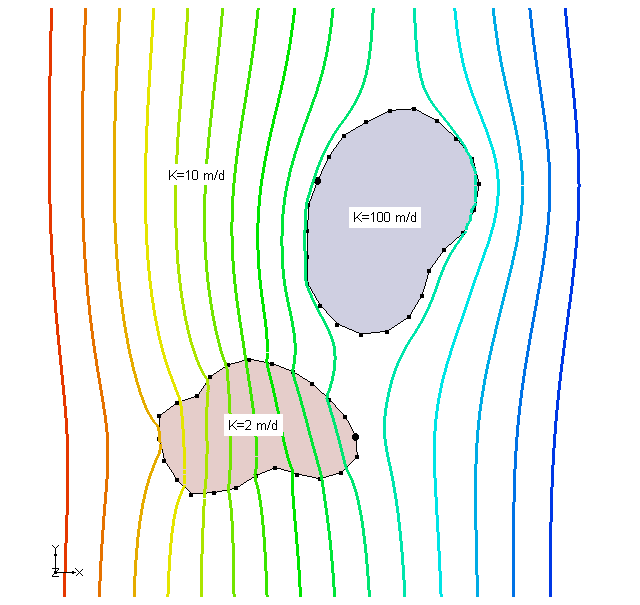
\includegraphics[width=6in,keepaspectratio,bb = 0 0 200 100, draft, type=eps]{figures/in0-polys.PNG}
	\end{centering}
	\caption{\label{cap:in0-polys}Potentiometric countours for two polygonal hydraulic conductivity inhomogeneities in a field of uniform flow. Flow is from left to right (red contours represent higher potentiometric heads). The domains are specified as follows: domain 0 (the outside) has $K=10\, m/d$; domain 1 has $K=100\, m/d$ and is shaded in blue; domain \#2 has $K=2\, m/d$ and is shaded in beige. No string specifications (\textsf{str} directive) were required.}
\end{figure}
\begin{figure}
	\begin{centering}
	%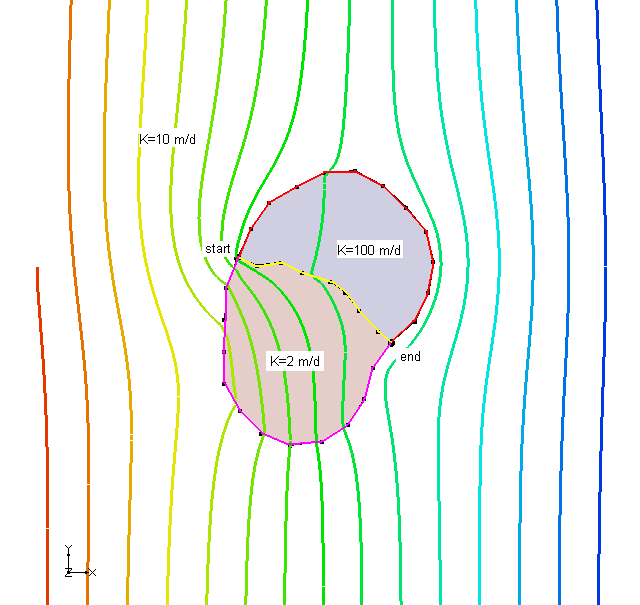
\includegraphics[width=6in,keepaspectratio,bb = 0 0 200 100, draft, type=eps]{figures/in0-strings.PNG}
	\end{centering}
	\caption{\label{cap:in0-strings}Potentiometric countours for two polygonal hydraulic conductivity inhomogeneities with a common boundary in a field of uniform flow. Flow from left to right (red contours represent higher heads). The domains are specified as follows: domain 0 (the outside) has $K=10\, m/d$; domain 1 has $K=100\, m/d$ and is shaded in blue; domain \#2 has $K=2\, m/d$ and is shaded in beige. Three strings are required; all share the same starting and ending points. The three strings are specified as follows: string 1 (red) has $left=0$, $right=1$; string 2 (yellow) has $left=1$; $right=2$; string 3 (purple) has $left=2$, $right=0$.}
\end{figure}
The following properties may be changed in ModAEM inhomogeneities:
\begin{itemize}
\item Hydraulic conductivity, $K$
\item Aquifer base elevation, $b$ 
\item Aquifer thickness, $H$
\item Aquifer effective porosity, $n$
\end{itemize}
In the case where base elevation and aquifer thickness are constant throughout the model domain, or when the flow is confined everywhere in the model, the equations solved by ModAEM for inhomogeneities are linear; only a few iterations are needed to achieve an accurate solution. In the case where the base elevation or aquifer thickness varies \emph{and} there are regions within the model where the flow is unconfined, the solution matrix contains coefficients that are dependent on the saturated thickness; additional iterations are required to achieve an accurate solution. For this reason, each sub-domain in the model has an additional parameter, the "initial average head''. The initial average head is the modeler's best estimate for the average head in the sub-domain. It is used to compute the saturated thickness during the first model iteration. Obviously, a good estimate for the initial average head helps the model stability.

\subsection{Specifying inhomogeneities}

As mentioned above, ModAEM allows for both closed polygonal inhomogeneities that do not share edges and for complex polygonal inhomogeneities that may have shared edges. ModAEM requires that the specification of inhomogeneities be done in two steps:
\begin{enumerate}
\item Defining the polygonal regions using the \textsf{dom} directive
\item Where necessary, defining the strings of elements that implement the boundaries using the \textsf{str} directive.
\end{enumerate}
Task (2) can be very complicated. Fortunately there are preprocessing tools such as GMS (EMS-I) and ArcInfo that provide an ``arc--node'' data representation to make it simpler. For many problems, inhomogeneities with common boundaries are unnecessary. Fortunately, ModAEM makes it easier to specify these (see below).

\paragraph{Usage:}
\begin{verbatim}
aqu ndomains nstrings base ...
  in0
    dom nvertices bot thick hyd-cond poro avg-head id
      (x1,y1)
      (x2,y2)
      ...
    dom ...
      ...
    str nvertices left right id
      (x1,y1)
      (x2,y2)
      ...
    str ...
      ...
  end
end
\end{verbatim}
As noted above, the maximum number of domains and strings to be used are specified in the \textsf{aqu} directive that begins the aquifer specification. The specification of inhomogeneities begins with the \textsf{in0} directive, which enters the inhomogeneity specification section of the ModAEM script file. Inside the IN0 section of the script, domains are specified first, then strings are defined that actually implement the boundaries\footnote{For problems without common boundaries, no string definitions are required; ModAEM automatically builds strings for closed domains.}.

\paragraph{Parameters for domain specification (directive \textsf{dom})}
\begin{description}
\item [{\texttt{nvertices}} (int)] The maximum number of vertices which may be used to delineate the boundary of the domain. $[-]$
\item [{\texttt{base}} (real)] The base elevation of the aquifer $[\mathrm{L}]$
\item [{\texttt{thickness}} (real)] The thickness of the aquifer $[\mathrm{L}]$
\item [{\texttt{conductivity}} (real)] The hydraulic conductivity (real) of the aquifer $[\mathrm{L/T}]$
\item [{\texttt{porosity}} (real)] Porosity of the aquifer as a fraction $[-]$
\item [{\texttt{initial-avg-head}} (real)] This is an estimate of the average head in the aquifer. It is used to pre--condition the solution when inhomogeneities in base elevation or thickness are encountered and the flow condition is unconfined. If you expect to be using inhomogeneities in base elevation or aquifer thickness, a good estimate of the initial average head will greatly speed the solution process. If you are not using inhomogeneities in base elevation or aquifer thickness, it is recommended that the value of $\mathtt{base+thickness}$ be provided. $[\mathrm{L}]$
$\{real\}$
As usual, flow may be confined and/or unconfined within the domain. If the flow is unconfined, additional iterations may be required for an accurate solution.
\item [{\texttt{id}} (int)] A unique identification number for the domain.
\end{description}

\paragraph{Specifying the vertices along the domain perimeter}
Following the \textsf{dom} directive, up to \texttt{nvertices} vertices may be provided, one vertex per line in the input file. Each vertex is a single complex coordinate. Each vertex is entered as a single complex coordinate, $\mathtt{(x_p, y_p)}$, where $p$ is the index of the vertex along the perimeter, $z_{p}=x_{p}+y_{p}$ $[\mathrm{L}]$


\paragraph{Parameters for string specification (directive \textsf{\textmd{str}})}

As mentioned above, ModAEM makes things easier for modelers who build input files by hand or from shapefiles that do not support an ``arc/node'' spatial data structure. If no common boundaries are to be specified, e.g. as in Figure \ref{cap:in0-polys}, the \textsf{str} directive should be omitted. ModAEM will automatically build closed strings of elements. The following describes the input format for inhomogeneity strings (please refer to Figure \ref{cap:in0-strings}).
\begin{description}
\item [{\texttt{nvertices}} (int)] The maximum number of vertices which may be used to delineate the string. $[-]$
\item [{\texttt{left}} (int)] The ID number of the polygon that is to the left of the string (see section \ref{sec:The-right--hand-rule}). $[-]$
\item [{\texttt{right}} (int)] The ID number of the polygon that is to the left of the string (see section \ref{sec:The-right--hand-rule}). $[-]$
\item [{\texttt{closed}} (logical)] Flag; if true, the string closes on itself, making a polygon. If false, the string is an open polyline. $[-]$
\item [{\texttt{id}} (int)] A unique identification number for the string. $[-]$
\end{description}